\documentclass[xcolor=dvipsnames]{beamer}

\usepackage[orientation=landscape,size=a0,scale=1.4,debug]{beamerposter}


%\mode<presentation>
\usetheme{PGRposter}



\usepackage{cite}
\usepackage{amsmath,amssymb,amsfonts}
%\usepackage{amsthm, latexsym}
\usepackage{algorithmic}
\usepackage{graphicx}
\usepackage{textcomp}
\usepackage{bm}
\usepackage{upgreek}

\usepackage[retainorgcmds]{IEEEtrantools}

%\usepackage{hyperref}

%\usepackage[english]{babel}

\usepackage{hhline}



\DeclareMathOperator{\xrm}{\mathrm{x}}
\DeclareMathOperator{\Xrm}{\mathrm{X}}
\DeclareMathOperator{\yrm}{\mathrm{y}}
\DeclareMathOperator{\Yrm}{\mathrm{Y}}
\DeclareMathOperator{\Drm}{\mathrm{D}}
\DeclareMathOperator{\nrm}{\mathrm{n}}
\DeclareMathOperator{\nbarrm}{\bar{\mathrm{n}}}
\DeclareMathOperator{\zrm}{\mathrm{z}}

\DeclareMathOperator{\Prm}{\mathrm{P}}
\DeclareMathOperator{\prm}{\mathrm{p}}
\DeclareMathOperator{\Erm}{\mathrm{E}}
\DeclareMathOperator{\Crm}{\mathrm{C}}

\DeclareMathOperator{\Xcal}{\mathcal{X}}
\DeclareMathOperator{\Ycal}{\mathcal{Y}}
\DeclareMathOperator{\Dcal}{\mathcal{D}}
\DeclareMathOperator{\Ncal}{\mathcal{N}}
\DeclareMathOperator{\Zcal}{\mathcal{Z}}
\DeclareMathOperator{\Hcal}{\mathcal{H}}
\DeclareMathOperator{\Fcal}{\mathcal{F}}
\DeclareMathOperator{\Rcal}{\mathcal{R}}
\DeclareMathOperator{\Mcal}{\mathcal{M}}
\DeclareMathOperator{\Scal}{\mathcal{S}}
\DeclareMathOperator{\Pcal}{\mathcal{P}}
\DeclareMathOperator{\Lcal}{\mathcal{L}}

\DeclareMathOperator{\Rbb}{\mathbb{R}}
\DeclareMathOperator{\Nbb}{\mathbb{N}}
\DeclareMathOperator{\Zbb}{\mathbb{Z}}

\DeclareMathOperator{\Dir}{\mathrm{Dir}}
\DeclareMathOperator{\DM}{\mathrm{DM}}
\DeclareMathOperator{\Multi}{\mathrm{Multi}}
\DeclareMathOperator{\DP}{\mathrm{DP}}




\graphicspath{ {../Figures/} }




\title[Predictive Distribution Estimation]{\uppercase{Predictive Distribution Estimation for Bayesian Machine Learning using a Dirichlet Process Prior}}
\author[Rademacher \& Doroslova\v{c}ki]{Paul Rademacher\inst{1} and Milo\v{s} Doroslova\v{c}ki\inst{2}}
\institute[NRL,~GWU] 
{
  \inst{1}
  Radar Division,~U.S. Naval Research Laboratory
  ;~
  \inst{2}
  Department of Electrical and Computer Engineering,~The George Washington University
}

\date{November 6, 2019}

%\logo{\includegraphics[width=8cm]{avatar.jpg}}
%\logo{\includegraphics[width=10cm]{C:/Users/paulg/Pictures/logo_NRL.png}}
%\logo{\includegraphics[width=10cm]{C:/Users/paulg/Pictures/gw_primary_2c_rev.png}}



\begin{document}

\begin{frame}{}


\begin{columns}[T]
%\begin{columns}[T, totalwidth=\textwidth]



%%% Column One
\begin{column}{.29\linewidth}
     
\begin{block}{Overview}
	
\begin{itemize}
\item In Bayesian treatments of machine learning, the success or failure of the estimator/classifier hinges on how well the prior distribution selected by the designer matches the actual data-generating model
\item Highly localized Dirichlet priors can overcome the burden of a limited training set when the prior mean is well matched to the true distribution, but will degrade the approximation if the match is poor
\end{itemize}
	
\end{block}


\begin{block}{Objective}

\textbf{Make inferences about unobservable $\yrm \in \Ycal$ given observed $\xrm \in \Xcal$ and a training set $\Drm \in \Dcal = \{\Ycal \times \Xcal\}^N$}


\vspace{1cm}


\begin{itemize}
\item Joint elements $(\yrm,\xrm)$ and $\Drm_n$ are distributed by an \emph{unknown} PMF $\theta$:
\begin{IEEEeqnarray}{rCl}
\Prm_{\yrm,\xrm,\Drm | \uptheta}(y,x,D | \theta) & = & \Prm_{\yrm,\xrm | \uptheta}(y,x | \theta) \prod_{n=1}^N \Prm_{ \Drm_n | \uptheta }\big( D_n | \theta \big) \nonumber \\
& = & \theta(y,x) \prod_{y' \in \Ycal} \prod_{x' \in \Xcal} \theta(y',x')^{\bar{N}(y',x';D)} \nonumber
\end{IEEEeqnarray}
\item $\Prm_{\Drm | \uptheta}$ depends on $\Drm$ only through the transform $\bar{N}(y,x;D) \equiv \sum_{n=1}^N \delta \big[ (y,x),D_n \big]$
\begin{itemize}
\item[$\Rightarrow$] Random process $\nbarrm \equiv \bar{N}(\Drm) \in \bar{\Ncal}$ is a \underline{sufficient statistic} for $\theta$; decisions can depend on $\nbarrm$ in place of $\Drm$
\end{itemize}
\end{itemize}
% + \delta[y',y]\delta[x'.x]

\hrulefill

\vspace{1cm}

Design a decision function $f: \bar{\Ncal} \mapsto \Hcal^{\Xcal}$, where $\Hcal$ is the decision space. 

The metric is a loss function $\Lcal: \Hcal \times \Ycal \mapsto \Rbb_{\geq 0}$.

\vspace{1cm}


\underline{Clairvoyant Risk}:
\begin{equation*} \label{eq:risk_cond}
\Rcal_{\uptheta}(f) = \Erm_{\xrm,\nbarrm | \uptheta} \bigg[ \Erm_{\yrm | \xrm,\uptheta} \Big[ \Lcal\big( f(\xrm;\nbarrm),\yrm \big) \Big] \bigg] 
\end{equation*}

\begin{itemize}
\item[$\Rightarrow$] Optimal decisions depend on the \emph{true predictive distribution}, $\Prm_{\yrm | \xrm,\uptheta} = \uptheta(\cdot,\xrm) / \sum_{y \in \Ycal} \uptheta(y,\xrm) \equiv \tilde{\uptheta}(\xrm)$
\end{itemize}


\large
\begin{equation*} 
\Downarrow \quad \Downarrow \quad \textbf{\textit{Select Prior }} \bm{\mathrm{p}_\uptheta} \quad \Downarrow \quad \Downarrow 
\end{equation*}
\normalsize

\vspace{1em}

\underline{Bayes Risk}:
\begin{IEEEeqnarray}{C} \label{eq:risk}
\Rcal(f) = \Erm_{\uptheta}\Big[ \Rcal_{\uptheta}\big( f(\xrm;\nbarrm) \big) \Big] = \Erm_{\xrm,\nbarrm}\bigg[ \Erm_{\yrm | \xrm,\nbarrm} \Big[ \Lcal\big( f(\xrm;\nbarrm),\yrm \big) \Big] \bigg] \nonumber
\end{IEEEeqnarray}

\begin{itemize}
\item[$\Rightarrow$] Decisions formulated using \emph{Bayes predictive distribution}, $\Prm_{\yrm | \xrm,\nbarrm} = \Erm_{\uptheta | \xrm,\nbarrm} \big[ \Prm_{\yrm | \xrm,\uptheta} \big] = \mu_{\tilde{\uptheta}(\xrm) | \xrm,\nbarrm}$
\end{itemize}

	
\end{block}
        
\end{column}




%%% Column Two
\begin{column}{.34\linewidth}
      
\begin{block}{Bayesian Prediction}

\begin{columns}[c]
\begin{column}{.49\linewidth}

\underline{Dirichlet Priors}:

%\vspace{1cm}

%\begin{IEEEeqnarray}{rCl}
%\prm_\uptheta(\theta) & = & \Dir(\theta;\alpha) \nonumber \\
%& = & \beta(\alpha)^{-1} \prod_{y \in \Ycal} \prod_{x \in \Xcal} \theta(y,x)^{\alpha(y,x) - 1} \nonumber \\
%& \Downarrow & \nonumber \\
%\prm_{\tilde{\uptheta}}\big(\tilde{\theta}\big) & = & \prod_{x \in \Xcal} \Dir\big(\tilde{\theta}(x);\alpha(\cdot,x)\big) \nonumber
%\end{IEEEeqnarray}

%\begin{IEEEeqnarray}{rCl}
%\prm_\uptheta(\theta) & = & \Dir(\theta;\alpha) \nonumber \\
%& = & \beta(\alpha)^{-1} \prod_{y \in \Ycal} \prod_{x \in \Xcal} \theta(y,x)^{\alpha(y,x) - 1} \nonumber \\
%& \Downarrow & \nonumber \\
%\prm_{\tilde{\uptheta}(x)}\big(\tilde{\theta}(x)\big) & = & \Dir\big(\tilde{\theta}(x);\alpha(\cdot,x)\big) \nonumber
%\end{IEEEeqnarray}

\begin{IEEEeqnarray}{rCl}
\prm_\uptheta(\theta) & = & \Dir(\theta;\alpha) \nonumber \\
& = & \beta(\alpha)^{-1} \prod_{y \in \Ycal} \prod_{x \in \Xcal} \theta(y,x)^{\alpha(y,x) - 1} \nonumber 
\end{IEEEeqnarray}
\large \begin{equation*} \Downarrow \end{equation*} \normalsize
\begin{IEEEeqnarray}{rCl}
\prm_{\tilde{\uptheta}}\big(\tilde{\theta}\big) & = & \prod_{x \in \Xcal} \Dir\big(\tilde{\theta}(x);\alpha(\cdot,x)\big) \nonumber
\end{IEEEeqnarray}

\vspace{1cm}

\begin{itemize}
\item Concentration parameters $\alpha'(x) \equiv \sum_{y \in \Ycal} \alpha(y,x)$ enable both \emph{subjective} and \emph{non-informative} priors
\item Conjugate Prior for I.I.D. observations $\Rightarrow$ Tractable Posterior
\end{itemize}



\end{column}
\begin{column}{.44\linewidth}


\begin{figure}
\centering
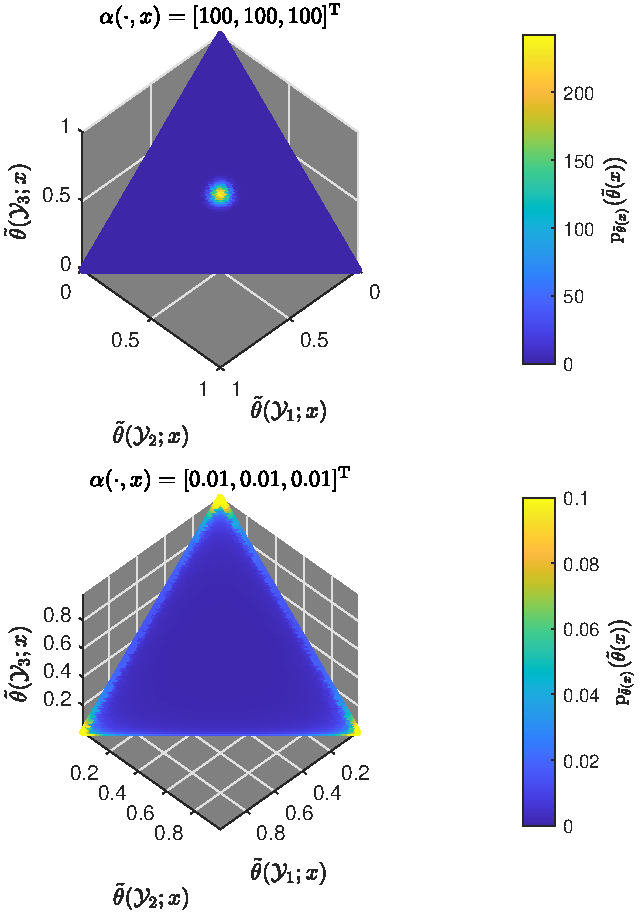
\includegraphics[width=0.9\linewidth]{P_theta_tilde.pdf}
%\caption{Model prior PDF for different concentrations $\alpha'(x)$}
%\label{fig:P_theta}
\end{figure}

\end{column}
\end{columns}



\vspace{1cm}

\hrulefill

\vspace{1cm}



\begin{columns}[c]
\begin{column}{.49\linewidth}

\underline{Dirichlet Posteriors}:

\begin{IEEEeqnarray}{L}
\prm_{\tilde{\uptheta} | \xrm,\nbarrm}(\tilde{\theta} | x,\bar{n}) = \prm_{\tilde{\uptheta} | \nbarrm}(\tilde{\theta} | \bar{n}) \nonumber \\
= \prod_{x' \in \Xcal} \prm_{\tilde{\uptheta}(x') | \nbarrm(\cdot,x')}\big(\tilde{\theta}(x') | \bar{n}(\cdot,x') \big)) \nonumber \\
= \prod_{x' \in \Xcal} \Dir\big( \tilde{\theta}(x') ; \alpha(\cdot,x') + \bar{n}(\cdot,x') \big) \nonumber 
\end{IEEEeqnarray}


\vspace{1cm}

\begin{itemize}
\item \textbf{Full support} over distribution space ensures identification of model $\tilde{\uptheta}(x)$ as $n'(x) \equiv \sum_y \bar{n}(y,x) \to \infty$
\end{itemize}


\end{column}
\begin{column}{.44\linewidth}

\begin{figure}
\centering
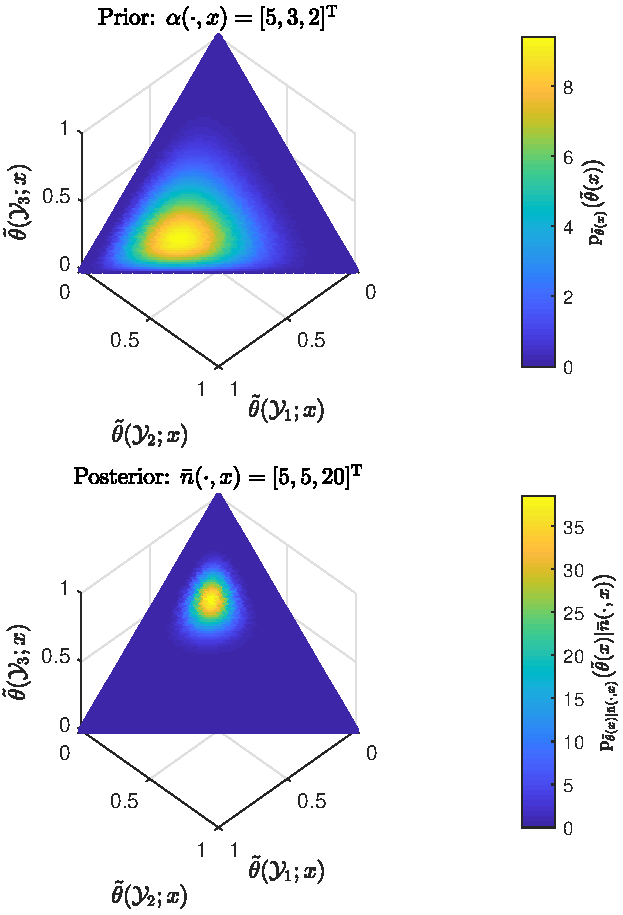
\includegraphics[width=0.9\linewidth]{P_theta_post_tilde.pdf}
%\caption{Model $\uptheta$ PDF, prior and posterior}
%\label{fig:P_theta_D}
\end{figure}

\end{column}
\end{columns}


\vspace{1cm}

\hrulefill

\vspace{1cm}

\underline{\textbf{Bayes Predictive Distribution}}:

\begin{IEEEeqnarray}{rCl}
\Prm_{\yrm | \xrm,\nbarrm} & = & \left(\frac{\alpha'(\xrm)}{\alpha'(\xrm) + \sum_y \nbarrm(y,\xrm)}\right) \frac{\alpha(\cdot,\xrm)}{\alpha'(\xrm)} + \left(\frac{\sum_y \nbarrm(y,\xrm)}{\alpha'(\xrm) + \sum_y \nbarrm(y,\xrm)}\right) \frac{\nbarrm(\cdot,\xrm)}{\sum_y \nbarrm(y,\xrm)} \nonumber 
\end{IEEEeqnarray}

\vspace{1cm}

\begin{itemize}
\item[$\Rightarrow$] Convex combination of data-independent PMF and conditional empirical PMF
\item[$\Rightarrow$] $\Erm_{\nbarrm | \nrm',\uptheta}\big[ \Prm_{\yrm | \xrm,\nbarrm} \big] = \left(\frac{\alpha'(\xrm)}{\alpha'(\xrm) + \nrm'(\xrm)}\right) \frac{\alpha(\cdot,\xrm)}{\alpha'(\xrm)} + \left(\frac{\nrm'(\xrm)}{\alpha'(\xrm) + \nrm'(\xrm)}\right) \tilde{\uptheta}(\xrm)$
\end{itemize}

%\begin{IEEEeqnarray}{L}
%\Erm_{\nbarrm | \nrm',\uptheta}\big[ \Prm_{\yrm | \xrm,\nbarrm} \big] = \left(\frac{\alpha'(\xrm)}{\alpha'(\xrm) + \nrm'(\xrm)}\right) \frac{\alpha(\cdot,\xrm)}{\alpha'(\xrm)} + \left(\frac{\nrm'(\xrm)}{\alpha'(\xrm) + \nrm'(\xrm)}\right) \tilde{\uptheta}(\xrm) \nonumber 
%\end{IEEEeqnarray}


\end{block}  
    
\end{column}





%%% Column Three
\begin{column}{.34\linewidth}
      
\begin{block}{Density Estimation}

\begin{columns}[c]
\begin{column}{.53\linewidth}
%\centering 

\begin{itemize}
\item[$*$] Density estimation accuracy assessed using the \emph{Estimation Difference Function}:
\end{itemize}

%Density estimation accuracy assessed using first and second moments of the \emph{Estimation Difference Function}: 
\begin{equation*}
\Delta(\xrm,\nbarrm,\uptheta) \equiv \Prm_{\yrm | \xrm,\nbarrm} - \Prm_{\yrm | \xrm,\uptheta} \in \Rbb^{\Ycal}
\end{equation*}

\vspace{1cm}

%\begin{itemize}
%\item[$*$] First and second moments of $\Delta$ evaluated with respect to $\Prm_{\nbarrm | \nrm',\uptheta}$
%\end{itemize}


\end{column}
\begin{column}{.43\linewidth}

\begin{figure}
\centering
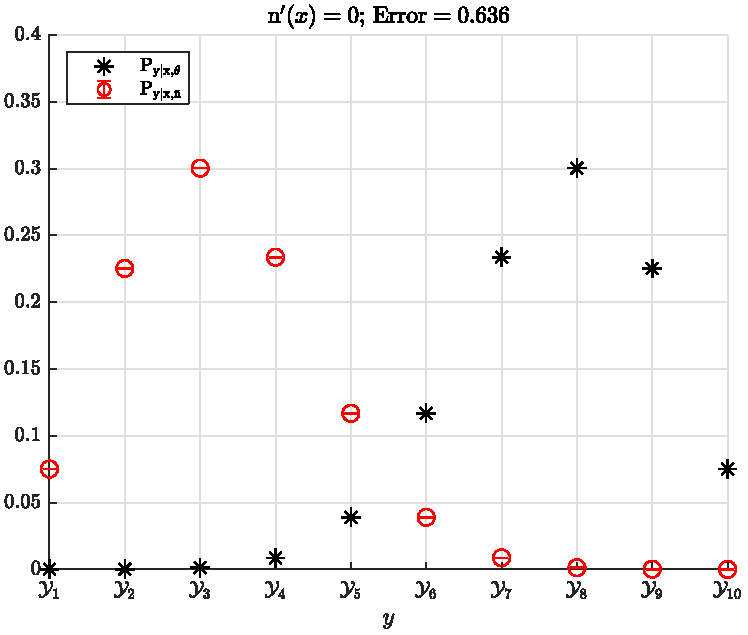
\includegraphics[width=0.8\linewidth]{P_yx_error_N_0.pdf}
%\caption{Model $\tilde{\uptheta}(x)$ estimate, $N=0$}
%\label{fig:P_yx_error_N_0}
\end{figure}

\end{column}
\end{columns}


\vspace{1cm}

\begin{IEEEeqnarray}{C} 
\mathrm{Bias}(\xrm,\nrm',\uptheta) = \Erm_{\nbarrm | \nrm',\uptheta}\big[ \Delta(\xrm,\nbarrm,\uptheta) \big] = \frac{\alpha'(\xrm)}{\alpha'(\xrm) + \nrm'(\xrm)} \left( \frac{\alpha(\cdot,\xrm)}{\alpha'(\xrm)} - \tilde{\uptheta}(\xrm) \right) \nonumber 
\end{IEEEeqnarray}
\begin{IEEEeqnarray}{rCl} 
\mathrm{Cov}(y,y';\xrm,\nrm',\uptheta) & = & \Crm_{\nbarrm | \nrm',\uptheta} \big[\Prm_{\yrm | \xrm,\nbarrm}(\cdot | \xrm,\nbarrm) \big](y,y') \nonumber \\
& = & \frac{\nrm'(\xrm)}{\big( \alpha'(\xrm) + \nrm'(\xrm) \big)^2} \left( \tilde{\uptheta}(y;\xrm) \delta[y,y'] - \tilde{\uptheta}(y;\xrm) \tilde{\uptheta}(y';\xrm) \right) \nonumber
\end{IEEEeqnarray}

%\vspace{1cm}
\large \begin{equation*} \Downarrow \quad \Downarrow \quad \Downarrow \end{equation*} \normalsize
\begin{IEEEeqnarray}{rCl} 
\mathcal{E}(y,y' ; \xrm,\nrm',\uptheta) & = & \Erm_{\nbarrm | \nrm',\uptheta} \Big[ \Delta(y;\xrm,\nbarrm,\uptheta) \Delta(y';\xrm,\nbarrm,\uptheta) \Big] \nonumber \\
& = & \bm{\mathrm{Bias}(y;\xrm,\nrm',\uptheta) \mathrm{Bias}(y';\xrm,\nrm',\uptheta) + \mathrm{Cov}(y,y';\xrm,\nrm',\uptheta)} \nonumber
\end{IEEEeqnarray}
%\begin{IEEEeqnarray}{L} 
%Error = \sqrt{\sum_{y \in \Ycal} \Erm_{\nbarrm | \nrm',\uptheta} \Big[ \Delta(y;\xrm,\nbarrm,\uptheta) \Delta(y;\xrm,\nbarrm,\uptheta) \Big]} \\
%= \bm{\sqrt{\sum_{y \in \Ycal} \mathrm{Bias}(y;\xrm,\nrm',\uptheta)^2 + \mathrm{Cov}(y,y;\xrm,\nrm',\uptheta)}} \nonumber
%\end{IEEEeqnarray}

\hrulefill

\vspace{0.5cm}

\begin{columns}[c]
\begin{column}{.48\linewidth}
\centering 

\begin{itemize}
\item[$*$] \large \textbf{Concentration parameter controls a \emph{Bias-Variance trade-off}} \normalsize
%\item $\mathrm{Error} = \sqrt{\sum_{y \in \Ycal} \mathcal{E}(y,y ; \xrm,\nrm',\uptheta)}$
\end{itemize}

\vspace{0.5cm}
$\mathrm{Error} = \sqrt{\sum_{y \in \Ycal} \mathcal{E}(y,y ; \xrm,\nrm',\uptheta)}$

\end{column}
\begin{column}{.48\linewidth}

\begin{table}
\renewcommand{\arraystretch}{1.5}
\begin{tabular}{| c | c | c |}
\hline 
$\alpha'(x)$ & Bias & Covariance \\
\hhline{|=|=|=|}
$\to \infty$ & $\frac{\alpha(\cdot,\xrm)}{\alpha'(\xrm)} - \tilde{\uptheta}(\xrm)$ & 0 \\ 
\hline
$\to 0$ & 0 & $\frac{\Sigma_{\nbarrm(\cdot,\xrm) | \nrm'(\xrm),\tilde{\uptheta}(\xrm)}(y,y')}{\nrm'(\xrm)^2}$ \\
\hline
\end{tabular}
%\caption{}
\end{table}

\end{column}
\end{columns}



\vspace{1cm}



\begin{columns}[t]
\begin{column}{.5\linewidth}

\begin{figure}
\centering
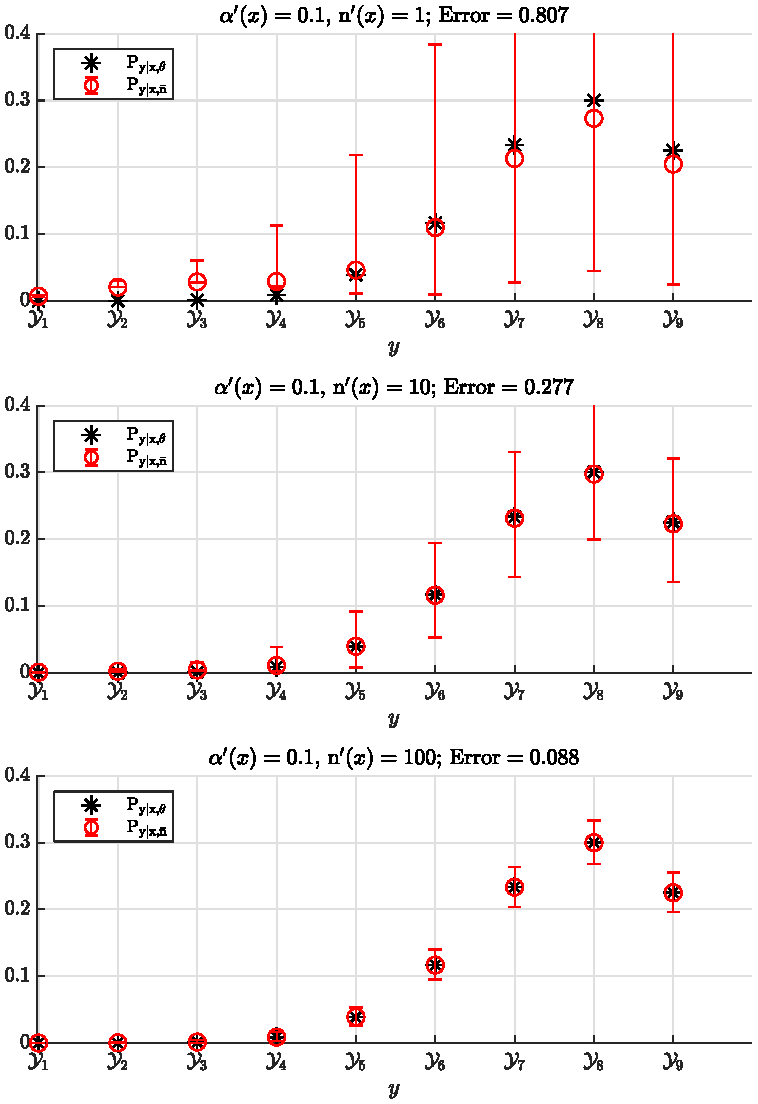
\includegraphics[width=0.9\linewidth]{P_yx_error_a0_0_1.pdf}
%\caption{Model $\tilde{\uptheta}(x)$ estimates, $\alpha'(x) = 0.1$}
%\label{fig:P_yx_error_a0_0_1}
\end{figure}

\end{column}
\begin{column}{.5\linewidth}

\begin{figure}
\centering
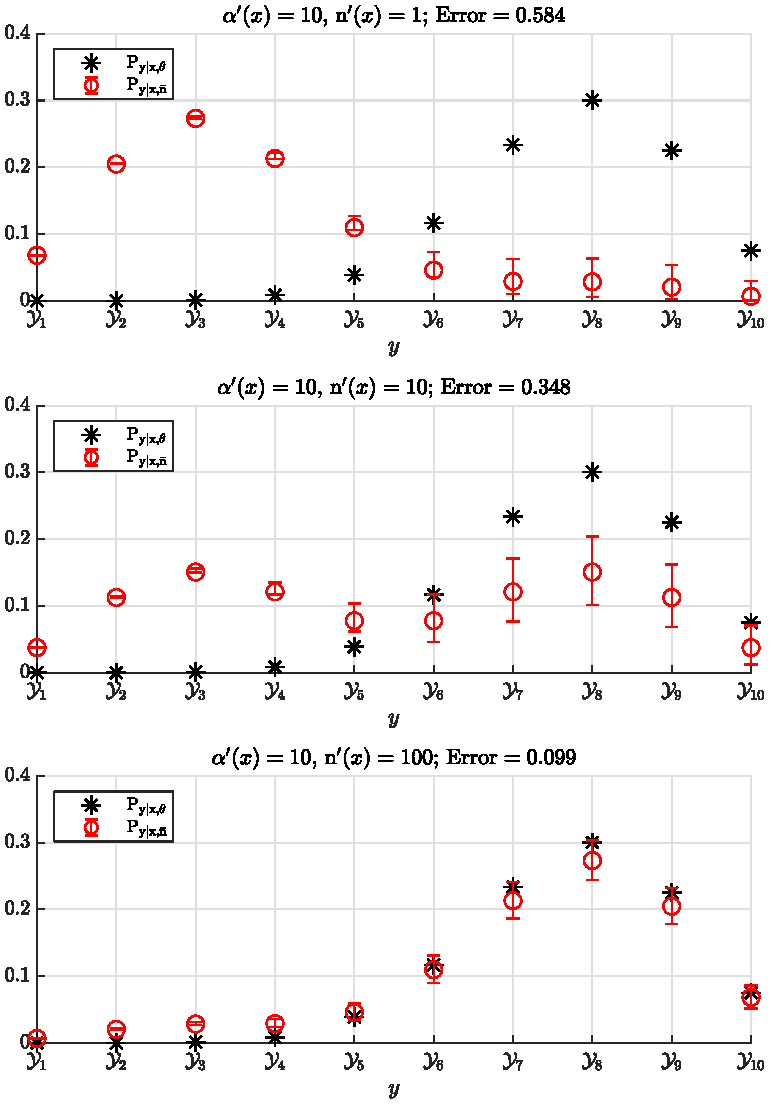
\includegraphics[width=0.9\linewidth]{P_yx_error_a0_10.pdf}
%\caption{Model $\tilde{\uptheta}(x)$ estimates, $\alpha'(x) = 10$}
%\label{fig:P_yx_error_a0_10}
\end{figure}

\end{column}
\end{columns}



\end{block}  
    
\end{column}




\end{columns}


\end{frame}


\end{document}



